%%%%%%%%%%%%%%%%%%%%%%%%%%%%%%%%%%%%%%%%%%%%%%%%%%%%%%%%%%%%%%%%%%%%%%%%%%%%%%%%%%
\begin{frame}[fragile]\frametitle{}
\begin{center}
{\Large Sequences}
\end{center}
\end{frame}

%%%%%%%%%%%%%%%%%%%%%%%%%%%%%%%%%%%%%%%%%%%%%%%%%%%%%%%%%%%%%%%%%%%%%%%%%%%%%%%%%%
\begin{frame}[fragile]\frametitle{}
\begin{center}
{\Large Lists}
\end{center}
\end{frame}

%%%%%%%%%%%%%%%%%%%%%%%%%%%%%%%%%%%%%%%%%%%%%%%%%%%%%%%%%%%%%%%%%%%%%%%%%%%%%%%%%%%
\begin{frame}[fragile]\frametitle{Built-in Sequences}

  \begin{itemize}
  \item {\bf list} \emph{mutable}, possibly heterogeneous
  \item{\bf tuple} \emph{immutable}, possibly heterogeneous
  \item{\bf str} \emph{immutable}, only holds characters
  \end{itemize}
\end{frame}


%%%%%%%%%%%%%%%%%%%%%%%%%%%%%%%%%%%%%%%%%%%%%%%%%%%%%%%%%%%%%%%%%%%%%%%%%%%%%%%%%%%
\begin{frame}[fragile]\frametitle{Sequences from Other Packages}
  \begin{itemize}
  \item \href{http://numpy.scipy.org}{NumPy}: {\bf array} \emph{mutable}, homogeneous (like C/Fortran arrays)
  \item Collections: OrderedDict
  \end{itemize}
\end{frame}

%%%%%%%%%%%%%%%%%%%%%%%%%%%%%%%%%%%%%%%%%%%%%%%%%%%%%%%%%%%%%%%%%%%%%%%%%%%%%%%%%%%
\begin{frame}[fragile]\frametitle{Lists}
  \begin{itemize}
  \item Ordered collections of arbitrary objects
  \item Accessed by offset
  \item Variable length, heterogeneous, arbitrarily nest-able
  \item Mutable sequence
  % \item Arrays of object references
  \end{itemize}
  \begin{lstlisting}
[10, 20, 30, 40]
['crunchy frog', 'ram bladder', 'lark vomit']
['spam', 2.0, 5, [10, 20]]
\end{lstlisting}
\end{frame}

%%%%%%%%%%%%%%%%%%%%%%%%%%%%%%%%%%%%%%%%%%%%%%%%%%%%%%%%%%%%%%%%%%%%%%%%%%%%%%%%%%%
\begin{frame}[fragile]\frametitle{List mutation}
Replace items by assigning them
  a new value:
\begin{lstlisting}
>>> L = ['U', 'Z', 'H']
>>> L[2] = 'G'
>>> print(L)
['U', 'Z', 'G']
\end{lstlisting}
Try negative indices.
\end{frame}

%%%%%%%%%%%%%%%%%%%%%%%%%%%%%%%%%%%%%%%%%%%%%%%%%%%%%%%%%%%%%%%%%%%%%%%%%%%%%%%%%%%
\begin{frame}[fragile]\frametitle{List mutation}

Replace an entire slice:
\begin{lstlisting}
>>> L[1:3] = ['a', 'b']
>>> print(L)
['U', 'a', 'b']
\end{lstlisting}
The range on the left is replaced by range on the right. If there is mismatch in the lengths? Try \ldots. 

Try negative ranges as well. If the range evaluates to null (L[-1:-2]) then right hand array is inserted at the -2 position?
\end{frame}


%%%%%%%%%%%%%%%%%%%%%%%%%%%%%%%%%%%%%%%%%%%%%%%%%%%%%%%%%%%%%%%%%%%%%%%%%%%%%%%%%%%
\begin{frame}[fragile]\frametitle{List mutation}
New slice does not need to have the same length:
\begin{lstlisting}
>>> L[2:] = range(4)
>>> print(L)
['U', 'a', 0, 1, 2, 3]
\end{lstlisting}
From 2 onwards there are only 1 (last) element, in its place put all of the right hand side, ie, array from 0 to 4.
\end{frame}

%%%%%%%%%%%%%%%%%%%%%%%%%%%%%%%%%%%%%%%%%%%%%%%%%%%%%%%%%%%%%%%%%%%%%%%%%%%%%%%%%%%
\begin{frame}[fragile]\frametitle{List mutation}
Add an element
\begin{lstlisting}
>>> L.append(4)
>>> L
['a', 0, 1, 2, 3, 4]
\end{lstlisting}
Return type of append() is None. It mutates the list itself. It does NOT return the modified list (like Strings).

So don't do:

\begin{lstlisting}
L = L.append(4)
\end{lstlisting}

\end{frame}

%%%%%%%%%%%%%%%%%%%%%%%%%%%%%%%%%%%%%%%%%%%%%%%%%%%%%%%%%%%%%%%%%%%%%%%%%%%%%%%%%%%
\begin{frame}[fragile]\frametitle{List mutation}
Remove individual items from a list either by specifying the item:
\begin{lstlisting}
>>> L.remove('U')
>>> L
['a', 0, 1, 2, 3, 4]
\end{lstlisting}
\end{frame}

%%%%%%%%%%%%%%%%%%%%%%%%%%%%%%%%%%%%%%%%%%%%%%%%%%%%%%%%%%%%%%%%%%%%%%%%%%%%%%%%%%%
\begin{frame}[fragile]\frametitle{List mutation}
or the position:

\begin{lstlisting}
>>> L.pop(1)
0
>>> L
['a', 1, 2, 3, 4]
\end{lstlisting}
\end{frame}

%%%%%%%%%%%%%%%%%%%%%%%%%%%%%%%%%%%%%%%%%%%%%%%%%%%%%%%%%%%%%%%%%%%%%%%%%%%%%%%%%%%
\begin{frame}[fragile]\frametitle{List mutation}

Note: \texttt{remove()} method only removes \textit{the first occurrence}:

\begin{lstlisting}
>>> L = ['a', 'b', 'a']
>>> L.remove('a')
>>> L
['b', 'a']
\end{lstlisting}

\end{frame}

%%%%%%%%%%%%%%%%%%%%%%%%%%%%%%%%%%%%%%%%%%%%%%%%%%%%%%%%%%%%%%%%%%%%%%%%%%%%%%%%%%%
\begin{frame}[fragile]\frametitle{List mutation}

``del'' operator can be used two ways:

Remoes definition of 2nd position, thus the list shrinks.

\begin{lstlisting}
>>> L = ['a', 'b', 'a']
>>> del L[1]
>>> L
['a', 'a']
\end{lstlisting}

Remove the definition of whole list:
\begin{lstlisting}
>>> del L
>>> L
"Not defined error"
\end{lstlisting}

\end{frame}

%%%%%%%%%%%%%%%%%%%%%%%%%%%%%%%%%%%%%%%%%%%%%%%%%%%%%%%%%%%%%%%%%%%%%%%%%%%%%%%%%%%
\begin{frame}[fragile]\frametitle{List Sorting}

Dont use old L.sort() method but newer sorted method.

Here sorted returns the copy of the sorted list keeping original intact.

\begin{lstlisting}
>>> L = [5,3,4,7]
>>> M = sorted(L)
>>> L
[5,3,4,7]
>>> M
[3,4,5,7]
\end{lstlisting}

\end{frame}

%%%%%%%%%%%%%%%%%%%%%%%%%%%%%%%%%%%%%%%%%%%%%%%%%%%%%%%%%%%%%%%%%%%%%%%%%%%%%%%%%%%
\begin{frame}[fragile]\frametitle{List Sorting}

Applies to strings also. The sorted() function can be customized through optional arguments. The sorted() optional argument reverse=True, e.g. sorted(list, reverse=True), makes it sort backwards.

\begin{lstlisting}
strs = ['aa', 'BB', 'zz', 'CC']
  print sorted(strs)  ## ['BB', 'CC', 'aa', 'zz'] (case sensitive)
  print sorted(strs, reverse=True)   ## ['zz', 'aa', 'CC', 'BB']
\end{lstlisting}

\end{frame}

%%%%%%%%%%%%%%%%%%%%%%%%%%%%%%%%%%%%%%%%%%%%%%%%%%%%%%%%%%%%%%%%%%%%%%%%%%%%%%%%%%%
\begin{frame}[fragile]\frametitle{List Custom Sorting With key=}

\begin{itemize}
\item For more complex custom sorting, sorted() takes an optional "key=" specifying a "key" function that transforms each element before comparison. The key function takes in 1 value and returns 1 value, and the returned "proxy" value is used for the comparisons within the sort.

\item For example with a list of strings, specifying key=len (the built in len() function) sorts the strings by length, from shortest to longest. The sort calls len() for each string to get the list of proxy length values, and then sorts with those proxy values.
\end{itemize}

\begin{lstlisting}
  strs = ['ccc', 'aaaa', 'd', 'bb']
  print sorted(strs, key=len)  ## ['d', 'bb', 'ccc', 'aaaa']
\end{lstlisting}

\begin{center}
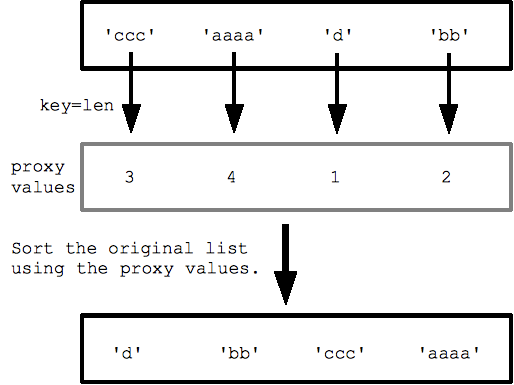
\includegraphics[width=0.6\linewidth,keepaspectratio]{custsort}
\end{center}

\tiny{(Ref: Google Python class)}
\end{frame}


%%%%%%%%%%%%%%%%%%%%%%%%%%%%%%%%%%%%%%%%%%%%%%%%%%%%%%%%%%%%%%%%%%%%%%%%%%%%%%%%%%%
\begin{frame}[fragile]\frametitle{Lists operators}
  You can concatenate two lists using the \texttt{+} operator:
  \begin{lstlisting}
>>> [1, 2] + [3, 4]
[1, 2, 3, 4]
  \end{lstlisting}
\end{frame}


%%%%%%%%%%%%%%%%%%%%%%%%%%%%%%%%%%%%%%%%%%%%%%%%%%%%%%%%%%%%%%%%%%%%%%%%%%%%%%%%%%%
\begin{frame}[fragile]\frametitle{Lists operators}
  You can mutate a list in place with the \texttt{+=} operator:
  \begin{lstlisting}
>>> L = [1, 2]
>>> L += [3, 4]
>>> print(L)
[1, 2, 3, 4]
  \end{lstlisting}
\end{frame}

%%%%%%%%%%%%%%%%%%%%%%%%%%%%%%%%%%%%%%%%%%%%%%%%%%%%%%%%%%%%%%%%%%%%%%%%%%%%%%%%%%%
\begin{frame}[fragile]\frametitle{Lists operators}
The \texttt{*} operator also works on lists:
  \begin{lstlisting}
>>> L = [1, 2]
>>> print(L*3)
[1, 2, 1, 2, 1, 2 ]
  \end{lstlisting}
\end{frame}

%%%%%%%%%%%%%%%%%%%%%%%%%%%%%%%%%%%%%%%%%%%%%%%%%%%%%%%%%%%%%%%%%%%%%%%%%%%%%%%%%%%
\begin{frame}[fragile]\frametitle{Traversing a list}
  Most common, for loop:
  \begin{lstlisting}
for cheese in cheeses:
    print(cheese)

for i in range(len(numbers)):
    numbers[i] = numbers[i] * 2
    
for x in empty:
	print('This never happens.')    
  \end{lstlisting}
\end{frame}



%%%%%%%%%%%%%%%%%%%%%%%%%%%%%%%%%%%%%%%%%%%%%%%%%%%%%%%%%%%%%%%%%%%%%%%%%%%%%%%%%%%
\begin{frame}[fragile]\frametitle{Exercise}
Take two lists, say for example these two:

  a = [1, 1, 2, 3, 5, 8, 13, 21, 34, 55, 89]
  b = [1, 2, 3, 4, 5, 6, 7, 8, 9, 10, 11, 12, 13]
  
and write a program that returns a list that contains only the elements that are common between the lists (without duplicates). Make sure your program works on two lists of different sizes.
\end{frame}

%%%%%%%%%%%%%%%%%%%%%%%%%%%%%%%%%%%%%%%%%%%%%%%%%%%%%%%%%%%%%%%%%%%%%%%%%%%%%%%%%%%
\begin{frame}[fragile]\frametitle{Lists and functions}
  \begin{lstlisting}
>>> nums = [3, 41, 12, 9, 74, 15]
>>> print(len(nums))
6
>>> print(max(nums))
74
>>> print(min(nums))
3
>>> print(sum(nums))
154
>>> print(sum(nums)/len(nums))
25
  \end{lstlisting}
\end{frame}

%%%%%%%%%%%%%%%%%%%%%%%%%%%%%%%%%%%%%%%%%%%%%%%%%%%%%%%%%%%%%%%%%%%%%%%%%%%%%%%%%%%
\begin{frame}[fragile]\frametitle{Average}
  \begin{lstlisting}
total = 0
count = 0

while (True):
	inp = input('Enter a number: ')
	if inp == 'done': break
	value = float(inp)
	total = total + value
	count = count + 1
	
average = total / count
print('Average:', average)
  \end{lstlisting}
\end{frame}


%%%%%%%%%%%%%%%%%%%%%%%%%%%%%%%%%%%%%%%%%%%%%%%%%%%%%%%%%%%%%%%%%%%%%%%%%%%%%%%%%%%
\begin{frame}[fragile]\frametitle{The `{\ttfamily\bfseries in}' operator}

  To test for presence of an item in a collection:

  \begin{itemize}
  \item {\bf x in S}:   Evaluates to \texttt{True} if \texttt{x} is equal to a \emph{value}
    contained in the \texttt{S} sequence (list, tuple, set).
\item {\bf x in T}: Evaluates to \texttt{True} if \texttt{x} is a substring of
    string \texttt{T}.
  \end{itemize}

\end{frame}


%%%%%%%%%%%%%%%%%%%%%%%%%%%%%%%%%%%%%%%%%%%%%%%%%%%%%%%%%%%%%%%%%%%%%%%%%%%%%%%%%%%
\begin{frame}[fragile]\frametitle{The \texttt{in} operator and the \texttt{if} conditional}

  Testing for the existence of an element in a container is a very
  common pattern:
  \texttt{in} operator:

\begin{lstlisting}
>>> L = [1, 2, 3, 4]
>>> if 1 in L:
...   print("Found!")
...
Found!
\end{lstlisting}
\end{frame}


%%%%%%%%%%%%%%%%%%%%%%%%%%%%%%%%%%%%%%%%%%%%%%%%%%%%%%%%%%%%%%%%%%%%%%%%%%%%%%%%%%%
\begin{frame}[fragile]\frametitle{The \texttt{in} operator and the \texttt{if} conditional}

Equivalent to the following, more verbose, less \textit{pythonic}:
 \begin{lstlisting}
 >>> L = [1, 2, 3, 4]
 >>> for item in L:
 ...     if item == 1:
 ...         print("Found!")
 ...         break
 \end{lstlisting}
\end{frame}


%%%%%%%%%%%%%%%%%%%%%%%%%%%%%%%%%%%%%%%%%%%%%%%%%%%%%%%%%%%%%%%%%%%%%%%%%%%%%%%%%%%
\begin{frame}[fragile]\frametitle{Zip and Argument Unpacking}
  \begin{itemize}
  \item zip transforms multiple lists into a single list of tuples
  \begin{lstlisting}
list1 = ['a', 'b', 'c']
list2 = [1, 2, 3]
zip(list1, list2) # is [('a', 1), ('b', 2), ('c', 3)]
  \end{lstlisting}
\item 	If the	lists are different lengths, zip stops as soon as the first list ends.
\item You can also unzip
  \begin{lstlisting}
pairs = [('a', 1), ('b', 2), ('c', 3)]
letters, numbers = zip(*pairs)
  \end{lstlisting}
\item The asterisk performs argument unpacking. Whats the ``type'' of ``letters'' and ``numbers''?
  \end{itemize}
\end{frame}

%%%%%%%%%%%%%%%%%%%%%%%%%%%%%%%%%%%%%%%%%%%%%%%%%%%%%%%%%%%%%%%%%%%%%%%%%%%%%%%%%%%
\begin{frame}[fragile]\frametitle{Lists and strings}
  \begin{itemize}
  \item String: sequence of characters
  \item List: sequence of values
  \item A list of characters is not the same as a string. 
  \item To convert from a string to a list of characters:
  \end{itemize}
    \begin{lstlisting}
>>> s = 'spam'
>>> t = list(s) #The list function breaks a string into individual letters.
>>> print(t)
['s', 'p', 'a', 'm']
  \end{lstlisting}
\end{frame}

%%%%%%%%%%%%%%%%%%%%%%%%%%%%%%%%%%%%%%%%%%%%%%%%%%%%%%%%%%%%%%%%%%%%%%%%%%%%%%%%%%%
\begin{frame}[fragile]\frametitle{Lists and strings}
  `Split' to break a string into list of words:
     \begin{lstlisting}
>>> s = 'pining for the fjords'
>>> t = s.split()
>>> print(t)
['pining', 'for', 'the', 'fjords']
>>> print(t[2])
  \end{lstlisting}
\end{frame}



%%%%%%%%%%%%%%%%%%%%%%%%%%%%%%%%%%%%%%%%%%%%%%%%%%%%%%%%%%%%%%%%%%%%%%%%%%%%%%%%%%%
\begin{frame}[fragile]\frametitle{Lists Exercise}
  \begin{itemize}
  \item Download www.py4e.com/code3/romeo.txt
  \item Open the file and read it line by line. 
  \item Split each line into a list of words using the split function.
  \item For each word, check to see if the word is already in a list. 
  \item If the word is not in the list, add it to the list.
  \item Sort and print the resulting words in alphabetical order.
  \end{itemize}
\end{frame}

%%%%%%%%%%%%%%%%%%%%%%%%%%%%%%%%%%%%%%%%%%%%%%%%%%%%%%%%%%%%%%%%%%%%%%%%%%%%%%%%%%%
\begin{frame}[fragile]\frametitle{Lists Exercise}
  \begin{lstlisting}
Enter file: romeo.txt
['Arise', 'But', 'It', 'Juliet', 'Who', 'already',
'and', 'breaks', 'east', 'envious', 'fair', 'grief',
'is', 'kill', 'light', 'moon', 'pale', 'sick', 'soft',
'sun', 'the', 'through', 'what', 'window',
'with', 'yonder']
  \end{lstlisting}
\end{frame}


%%%%%%%%%%%%%%%%%%%%%%%%%%%%%%%%%%%%%%%%%%%%%%%%%%%%%%%%%%%%%%%%%%%%%%%%%%%%%%%%%%%
\begin{frame}[fragile]\frametitle{Lists operations (recap)}
  \begin{itemize}
  \item empty list \lstinline{L = []}
  \item four items \lstinline{L2 = [0, 1, 2, 3]}
  \item nested \lstinline{L3 = ['abc', ['def', 'ghi']]}
  \item index \lstinline{L2[i], L3[i][j]}
  \item slice, length \lstinline{L2[i:j], len(L2)}
  \item concatenate, repeat \lstinline{L1 + L2, L2 * 3}
  \item iteration, membership \lstinline{for x in L2, 3 in L2}
  \item methods \lstinline{L2.append(4), L2.sort(), L2.index(1), L2.reverse()}
  \item shrinking \lstinline{del L2[k], L2[i:j] = []}
  \item assignment \lstinline{L2[i] = 1, L2[i:j] = [4,5,6]}
  \item create list \lstinline{range(4) # useful to loop}
  \end{itemize}
\end{frame}

%%%%%%%%%%%%%%%%%%%%%%%%%%%%%%%%%%%%%%%%%%%%%%%%%%%%%%%%%%%%%%%%%%%%%%%%%%%%%%%%%%
\begin{frame}[fragile]\frametitle{}
\begin{center}
{\Large Sequences: List Comprehensions}
\end{center}
\end{frame}

%%%%%%%%%%%%%%%%%%%%%%%%%%%%%%%%%%%%%%%%%%%%%%%%%%%%%%%%%%%%%%%%%%%%%%%%%%%%%%%%%%%
\begin{frame}[fragile]\frametitle{List Comprehensions}
  \begin{itemize}
  \item Compact syntax for \emph{filtering} elements  of a list and/or \emph{applying} a function to them.
\item To build a list.
\end{itemize}
Say, you wish to build a list of squares fro 0 to 5.
  \begin{lstlisting}
data = []
for num in range(6):
    data.append(num*num)
  \end{lstlisting}
  
 Can be written using \textit{list comprehension}:
  \begin{lstlisting}
data = [num*num for num in range(6) ]
  \end{lstlisting}

\end{frame}

%%%%%%%%%%%%%%%%%%%%%%%%%%%%%%%%%%%%%%%%%%%%%%%%%%%%%%%%%%%%%%%%%%%%%%%%%%%%%%%%%%%
\begin{frame}[fragile]\frametitle{List Comprehensions}
Say, you wish to build a list of squares fro 0 to 5, only for even numbers.
  \begin{lstlisting}
data = []
for num in range(6):
    if num%2==0:
        data.append(num*num)
  \end{lstlisting}
  
 Can be written using \textit{list comprehension}:
  \begin{lstlisting}
data = [num*num for num in range(6) if num%2==0 ]
  \end{lstlisting}

\end{frame}

%%%%%%%%%%%%%%%%%%%%%%%%%%%%%%%%%%%%%%%%%%%%%%%%%%%%%%%%%%%%%%%%%%%%%%%%%%%%%%%%%%%
\begin{frame}[fragile]\frametitle{Example: List Comprehensions}
 
Download  https://raw.github.com/gc3-uzh-ch/python-course/master/values.dat.

Build its list.
  \begin{lstlisting}
data = []
for num in open('values.dat').readlines():
    data.append(int(num))
  \end{lstlisting}
  
 Can be written using \textit{list comprehension}:
  \begin{lstlisting}
data = [ int(line) for line in open('values.dat').readlines() ]
  \end{lstlisting}

\end{frame}

%%%%%%%%%%%%%%%%%%%%%%%%%%%%%%%%%%%%%%%%%%%%%%%%%%%%%%%%%%%%%%%%%%%%%%%%%%%%%%%%%%%
\begin{frame}[fragile]\frametitle{List comprehensions}
  \def\e{\ttfamily\itshape}

  The general syntax of a list comprehension is:
  \begin{lstlisting}
    [expr for var in iterable if condition]
  \end{lstlisting}
  where:
  \begin{itemize}
  \item{\bf expr} is any Python expression;
  \item{\bf iterable} is a (generalized) sequence;
  \item {\bf condition} is a boolean expression, depending on
    {\e var};
  \item {\bf var} is a variable that will be bound in turn to each item
    in {\e iterable} which satisfies {\e condition}.
  \end{itemize}

   \textit{Create a new list, and for each \textbf{var} in the
    sequence \textbf{iterable}, if \textbf{condition} is true then add
    \textbf{expr} to the list.}
\end{frame}

%%%%%%%%%%%%%%%%%%%%%%%%%%%%%%%%%%%%%%%%%%%%%%%%%%%%%%%%%%%%%%%%%%%%%%%%%%%%%%%%%%%
\begin{frame}[fragile]\frametitle{List comprehensions}
Need not use all the values
  \begin{lstlisting}
zeros = [0 for _ in even_numbers] # just to have same size
  \end{lstlisting}
Mutliple for loops:
  \begin{lstlisting}
pairs = [(x,y)
		for x in range(10)
			for y in range(10)] # 100 pairs of [(0,0), (0,1)...]
  \end{lstlisting}
\end{frame}

%%%%%%%%%%%%%%%%%%%%%%%%%%%%%%%%%%%%%%%%%%%%%%%%%%%%%%%%%%%%%%%%%%%%%%%%%%%%%%%%%%%
\begin{frame}[fragile]\frametitle{Exercise}
  \begin{itemize}
  \item Write a program which will find all such numbers which are divisible by 7 but are not a multiple of 5,
between 2000 and 3200 (both included).
  \item The numbers obtained should be printed in a comma-separated sequence on a single line.
  \item Use ``join'' to make the single string. May need to cast integers by str() to be join-able.
  \end{itemize}  
\end{frame}

%%%%%%%%%%%%%%%%%%%%%%%%%%%%%%%%%%%%%%%%%%%%%%%%%%%%%%%%%%%%%%%%%%%%%%%%%%%%%%%%%%%
\begin{frame}[fragile]\frametitle{Exercise}
  \begin{itemize}
  \item Write a program that calculates and prints the value according to the given formula:
  \item Q = Square root of [(2 * C * D)/H]
  \item The fixed values of C and H: C is 50. H is 30.
  \item D is the variable whose values should be input to your program in a comma-separated sequence.
  \item Example: Let us assume the following comma separated input sequence is given to the program: 100,150,180
  \item The output of the program should be: 18,22,24
  \item Hints: If the output received is in decimal form, it should be rounded off to its nearest value (for example, if the output received is 26.0, it should be printed as 26)
%In case of input data being supplied to the question, it should be assumed to be a console input. 
  \end{itemize}  
\end{frame}

%%%%%%%%%%%%%%%%%%%%%%%%%%%%%%%%%%%%%%%%%%%%%%%%%%%%%%%%%%%%%%%%%%%%%%%%%%%%%%%%%%%
\begin{frame}[fragile]\frametitle{Solution}
  \begin{lstlisting}
import math
c=50
h=30
value = []
items=[x for x in input("Enter : ").split(',')]
for d in items:
    value.append(str(int(round(math.sqrt(2*c*float(d)/h)))))

print(','.join(value))
  \end{lstlisting}
\end{frame}



%%%%%%%%%%%%%%%%%%%%%%%%%%%%%%%%%%%%%%%%%%%%%%%%%%%%%%%%%%%%%%%%%%%%%%%%%%%%%%%%%%%
\begin{frame}[fragile]\frametitle{Exercise}
  \begin{itemize}
  \item Write a program that accepts a comma separated sequence of words as input and prints the words in a comma-separated sequence after sorting them alphabetically.
  \item Suppose the following input is supplied to the program:without,hello,bag,world
  \item Then, the output should be: bag,hello,without,world
%  \item Hints: In case of input data being supplied to the question, it should be assumed to be a console input.
  \end{itemize}  
\end{frame}

%%%%%%%%%%%%%%%%%%%%%%%%%%%%%%%%%%%%%%%%%%%%%%%%%%%%%%%%%%%%%%%%%%%%%%%%%%%%%%%%%%%
\begin{frame}[fragile]\frametitle{Solution}
  \begin{lstlisting}
items=[x for x in input("Enter : ").split(',')]
items.sort()
print(','.join(items))
  \end{lstlisting}
\end{frame}

%%%%%%%%%%%%%%%%%%%%%%%%%%%%%%%%%%%%%%%%%%%%%%%%%%%%%%%%%%%%%%%%%%%%%%%%%%%%%%%%%%%
\begin{frame}[fragile]\frametitle{Exercise}
  \begin{itemize}
  \item Write a program that accepts a sequence of whitespace separated words as input and prints the words after removing all duplicate words and sorting them alphanumerically.
  \item Suppose the following input is supplied to the program: hello world and practice makes perfect and hello world again
  \item Then, the output should be: again and hello makes perfect practice world
%  \item Hints: In case of input data being supplied to the question, it should be assumed to be a console input.
  \item We use set container to remove duplicated data automatically and then use sorted() to sort the data.
  \end{itemize}  
\end{frame}

%%%%%%%%%%%%%%%%%%%%%%%%%%%%%%%%%%%%%%%%%%%%%%%%%%%%%%%%%%%%%%%%%%%%%%%%%%%%%%%%%%%
\begin{frame}[fragile]\frametitle{Solution}
  \begin{lstlisting}
s = input("Enter : ")
words = [word for word in s.split(" ")]
print(" ".join(sorted(list(set(words)))))
  \end{lstlisting}
\end{frame}



%%%%%%%%%%%%%%%%%%%%%%%%%%%%%%%%%%%%%%%%%%%%%%%%%%%%%%%%%%%%%%%%%%%%%%%%%%%%%%%%%%%
\begin{frame}[fragile]\frametitle{Exercise}
  \begin{itemize}
  \item Write a program which takes 2 digits, X,Y as input and generates a 2-dimensional array. The element value in the i-th row and j-th column of the array should be i*j.
  \item Note:$ i=0,1 \ldots, X-1; j=0,1, \ldots Y-1.$
  \item Example: Suppose the following inputs are given to the program: 3,5
  \item Then, the output of the program should be: [[0, 0, 0, 0, 0], [0, 1, 2, 3, 4], [0, 2, 4, 6, 8]] 
  \item Hints: Note: In case of input data being supplied to the question, it should be assumed to be a console input in a comma-separated form.

  \end{itemize}  
\end{frame}

%%%%%%%%%%%%%%%%%%%%%%%%%%%%%%%%%%%%%%%%%%%%%%%%%%%%%%%%%%%%%%%%%%%%%%%%%%%%%%%%%%%
\begin{frame}[fragile]\frametitle{Solution}
  \begin{lstlisting}
input_str = input("Enter : ")
dimensions=[int(x) for x in input_str.split(',')]
rowNum=dimensions[0]
colNum=dimensions[1]
multilist = [[0 for col in range(colNum)] for row in range(rowNum)]

for row in range(rowNum):
    for col in range(colNum):
        multilist[row][col]= row*col

print(multilist)
  \end{lstlisting}
\end{frame}
%
%
%
%%%%%%%%%%%%%%%%%%%%%%%%%%%%%%%%%%%%%%%%%%%%%%%%%%%%%%%%%%%%%%%%%%%%%%%%%%%%%%%%%%%%
%\begin{frame}[fragile]\frametitle{Generators}
%  \begin{itemize}
%  \item List can grow big, very big, which can be a huge source of inefficiency, especially if you need only few values
%   \item Generator iterate over and produce as and when needed
%   \item Create using fucntion and keyword {\em yield}
%  \begin{lstlisting}
%def lazy_range(n):
%"""a lazy version of range"""
%i = 0
%while i < n:
%    yield i
%    i += 1
%  \end{lstlisting}
%\item Following loop will consume yielded voalues, one at a time until none are left:
%  \begin{lstlisting}
%for i in lazy_range(10):
%	do_something_with(i)
%  \end{lstlisting}
%\item Pythin has ready fiunction like that called {\em xrange()}
%  \end{itemize}
%\end{frame}
%
%%%%%%%%%%%%%%%%%%%%%%%%%%%%%%%%%%%%%%%%%%%%%%%%%%%%%%%%%%%%%%%%%%%%%%%%%%%%%%%%%%%%
%\begin{frame}[fragile]\frametitle{Randomness}
%  \begin{itemize}
%  \item Many times you need to use random numbers
%  \begin{lstlisting}
%import	random
%four_uniform_randoms = [random.random() for _ in range(4)]
%# [0.8444218515250481,	 # random.random() produces numbers
%# 0.7579544029403025,	# uniformly between 0 and 1
%# 0.420571580830845, #	it's the random function we'll use
%# 0.25891675029296335]	 # most often
%  \end{lstlisting}
%\item 	Actually produces pseudorandom	(that is, deterministic) numbers based on an internal state that you can set with random.seed	
%  \begin{lstlisting}
%random.seed(10) # set the seed to 10
%print random.random() # 0.57140259469 
%random.seed(10) # reset the seed to 10
%print random.random() # 0.57140259469 again
%  \end{lstlisting}
%  \end{itemize}
%\end{frame}
%
%
%%%%%%%%%%%%%%%%%%%%%%%%%%%%%%%%%%%%%%%%%%%%%%%%%%%%%%%%%%%%%%%%%%%%%%%%%%%%%%%%%%%%
%\begin{frame}[fragile]\frametitle{Exercises}
%\begin{itemize}
%\item
%    Write a function called \texttt{load\_data2(filename, bound)}
%    \item Use List  Comprehensions, 
%    \item Read  https://raw.github.com/gc3-uzh-ch/python-course/master/values.dat
%    \item Has one  integer number per line, and return a list of the integer values
%
%    \begin{lstlisting}
%>>> load_data2('values.dat', 300000)
%[299850, 299740, 299900, 299930]
%    \end{lstlisting}
%
% \end{itemize}
%\end{frame}

%
%%%%%%%%%%%%%%%%%%%%%%%%%%%%%%%%%%%%%%%%%%%%%%%%%%%%%%%%%%%%%%%%%%%%%%%%%%%%%%%%%%%%
%\begin{frame}[fragile]\frametitle{Exercises}
%\begin{itemize}
%\item Write a function \texttt{odd} that takes a list of integers and returns a list of all the odd ones.
%\item Write a function \texttt{concat} that takes a list of lists and
%    returns the concatenation of those lists. For instance:
%    \begin{lstlisting}
%>>> concat([ [1,2,3], [4,5,6], [7,8,9] ])
%[1, 2, 3, 4, 5, 6, 7, 8, 9]
%    \end{lstlisting}
%\end{itemize}
%
%
%\end{frame}


%%%%%%%%%%%%%%%%%%%%%%%%%%%%%%%%%%%%%%%%%%%%%%%%%%%%%%%%%%%%%%%%%%%%%%%%%%%%%%%%%%
\begin{frame}[fragile]\frametitle{}
\vspace{1in}
\begin{center}
{\Large Sequences: Tuples}
\end{center}
\end{frame}



%%%%%%%%%%%%%%%%%%%%%%%%%%%%%%%%%%%%%%%%%%%%%%%%%%%%%%%%%%%%%%%%%%%%%%%%%%%%%%%%%%%
\begin{frame}[fragile]\frametitle{Tuples}
  \begin{itemize}
  \item They are like lists but immutable. Why Lists and Tuples?
  \item When you want to make sure the content won't change.
  \end{itemize}
  \begin{lstlisting}
>>> T = (1, 2, 3)
>>> T[0]
1
>>> T[0:1]
(1,)
  \end{lstlisting}

\end{frame}



%%%%%%%%%%%%%%%%%%%%%%%%%%%%%%%%%%%%%%%%%%%%%%%%%%%%%%%%%%%%%%%%%%%%%%%%%%%%%%%%%%%
\begin{frame}[fragile]\frametitle{Tuples}
But they are \textit{immutable}

\begin{lstlisting}[basicstyle=\footnotesize\ttfamily]
>>> T[0] = 'a'
Traceback (most recent call last):
  File "<stdin>", line 1, in <module>
TypeError: 'tuple' object does not support item assignment
\end{lstlisting}
\end{frame}
%
%
%%%%%%%%%%%%%%%%%%%%%%%%%%%%%%%%%%%%%%%%%%%%%%%%%%%%%%%%%%%%%%%%%%%%%%%%%%%%%%%%%%%%
%\begin{frame}[fragile]\frametitle{Comparing tuples}
%The comparison operators work with tuples.
%\begin{lstlisting}[basicstyle=\footnotesize\ttfamily]
%>>> (0, 1, 2) < (0, 3, 4)
%True
%>>> (0, 1, 2000000) < (0, 3, 4)
%True
%    \end{lstlisting}
%\end{frame}
%
%
%
%%%%%%%%%%%%%%%%%%%%%%%%%%%%%%%%%%%%%%%%%%%%%%%%%%%%%%%%%%%%%%%%%%%%%%%%%%%%%%%%%%%%
%\begin{frame}[fragile]\frametitle{Comparing tuples}
%The sort function works the same way.
%    \begin{lstlisting}[basicstyle=\footnotesize\ttfamily]
%txt = 'but soft what light in yonder window'
%
%words = txt.split()
%
%t = list()
%
%for word in words:
%	t.append((len(word), word))
%	
%t.sort(reverse=True)
%
%res = list()
%for length, word in t:
%	res.append(word)
%	
%print(res)
%    \end{lstlisting}
%
%\end{frame}
%

%%%%%%%%%%%%%%%%%%%%%%%%%%%%%%%%%%%%%%%%%%%%%%%%%%%%%%%%%%%%%%%%%%%%%%%%%%%%%%%%%%%
\begin{frame}[fragile]
\frametitle{Multiple assignment}
You can assigning multiple variables at the same time
\begin{lstlisting}
>>> a, b, c = (1, 2, 3)
>>> print(a)
1
>>> print(b)
2
\end{lstlisting}
\end{frame}



%%%%%%%%%%%%%%%%%%%%%%%%%%%%%%%%%%%%%%%%%%%%%%%%%%%%%%%%%%%%%%%%%%%%%%%%%%%%%%%%%%%
\begin{frame}[fragile]
\frametitle{Multiple assignment}
It works with any sequence:

\begin{lstlisting}
>>> a, b, c = 'UZH'
>>> print(a)
U
\end{lstlisting}



  Can you think of a way to swap the values of two variables using this?


\begin{lstlisting}
>>> a, b = b, a
\end{lstlisting}
\end{frame}


%%%%%%%%%%%%%%%%%%%%%%%%%%%%%%%%%%%%%%%%%%%%%%%%%%%%%%%%%%%%%%%%%%%%%%%%%%%%%%%%%%%
\begin{frame}[fragile]\frametitle{Multiple assignment}
In \texttt{for}:
\begin{lstlisting}
>>> L = [(1,'a'), (2,'b'), (3, 'c')]
>>> for x, y in L:
...     print ("first is " + str(x)
...            + ' and second is ' + y)
\end{lstlisting}

  
Useful with functions that return a tuple.

``returning a comma separated elements creates a tuple. Multiple values can only be returned inside containers. It looks a bit peculiar, but it’s actually the comma that forms a tuple, not the parentheses''

\tiny{(Ref: How does Python return multiple values from a function? - Stack Overflow)}

\end{frame}

%%%%%%%%%%%%%%%%%%%%%%%%%%%%%%%%%%%%%%%%%%%%%%%%%%%%%%%%%%%%%%%%%%%%%%%%%%%%%%%%%%%
\begin{frame}[fragile]\frametitle{Clarify multiple return values with named tuples}
Is this good or bad? You don't know because it's not clear.
\begin{lstlisting}
# Old testmod return value
doctest.testmod()
# (0, 4)
\end{lstlisting}
Better:
\begin{lstlisting}
# New testmod return value, a namedTuple
doctest.testmod()
# TestResults(failed=0, attempted=4)
\end{lstlisting}

A namedTuple is a subclass of tuple so they still work like a regular tuple, but are more friendly. To make a namedTuple:
\begin{lstlisting}
TestResults = namedTuple('TestResults', ['failed', 'attempted'])
\end{lstlisting}

\tiny{(Ref: Transforming Code into Beautiful, Idiomatic Python -  Raymond Hettinger)}

\end{frame}

%%%%%%%%%%%%%%%%%%%%%%%%%%%%%%%%%%%%%%%%%%%%%%%%%%%%%%%%%%%%%%%%%%%%%%%%%%%%%%%%%%%
\begin{frame}[fragile]\frametitle{Unpacking sequences}
\begin{lstlisting}
p = 'Yogesh', 'Kulkarni', 0x30, 'python@example.com'

# A common approach / habit from other languages
fname = p[0]
lname = p[1]
age = p[2]
email = p[3]
\end{lstlisting}
Better:
\begin{lstlisting}
fname, lname, age, email = p
\end{lstlisting}

This approach uses tuple unpacking and is faster and more readable.

\tiny{(Ref: Transforming Code into Beautiful, Idiomatic Python -  Raymond Hettinger)}

\end{frame}

%%%%%%%%%%%%%%%%%%%%%%%%%%%%%%%%%%%%%%%%%%%%%%%%%%%%%%%%%%%%%%%%%%%%%%%%%%%%%%%%%%%
\begin{frame}[fragile]\frametitle{Exercise}
\begin{itemize}
\item Write a program which accepts a sequence of comma-separated numbers from console and generate a list and a tuple which contains every number.
\item Suppose the following input is supplied to the program: 34,67,55,33,12,98
\item Then, the output should be: ['34', '67', '55', '33', '12', '98'] ('34', '67', '55', '33', '12', '98')
%\item Hints: In case of input data being supplied to the question, it should be assumed to be a console input.
%tuple() method can convert list to tuple
\end{itemize}
\end{frame}

%%%%%%%%%%%%%%%%%%%%%%%%%%%%%%%%%%%%%%%%%%%%%%%%%%%%%%%%%%%%%%%%%%%%%%%%%%%%%%%%%%%
\begin{frame}[fragile]\frametitle{Solution}
\begin{lstlisting}
values=input("Enter : ")
l=values.split(",")
t=tuple(l)
print(l)
print(t)
\end{lstlisting}
\end{frame}

%%%%%%%%%%%%%%%%%%%%%%%%%%%%%%%%%%%%%%%%%%%%%%%%%%%%%%%%%%%%%%%%%%%%%%%%%%%%%%%%%%%%
%\begin{frame}[fragile]\frametitle{Exercises}
%
%  \begin{itemize}
%    \item
%    Implement a \texttt{zip2} function,
%    \item Takes a list of 2-tuples
%    \item Returns \emph{two} lists: 
%    \item list of all the first items in the
%    pairs, 
%    \item list of all the second items in the pairs.
%
%    \begin{lstlisting}
%>>> zip2( [('a', 1), ('b', 2), ('c', 3)] )
%(['a', 'b', 'c'], [1, 2, 3])
%    \end{lstlisting}
%\end{itemize}
%\end{frame}
%
%

%
%
%%%%%%%%%%%%%%%%%%%%%%%%%%%%%%%%%%%%%%%%%%%%%%%%%%%%%%%%%%%%%%%%%%%%%%%%%%%%%%%%%%%%
%\begin{frame}[fragile]\frametitle{Exercise}
%  \begin{itemize}
%  \item You are required to write a program to sort the (name, age, height) tuples by ascending order where name is string, age and height are numbers. The tuples are input by console. The sort criteria is:
%  \item 1: Sort based on name;
%  \item 2: Then sort based on age;
%  \item 3: Then sort by score.
%  \item The priority is that name > age > score.
%  \item If the following tuples are given as input to the program:
%    \begin{lstlisting}
%Tom,19,80
%John,20,90
%Jony,17,91
%Jony,17,93
%Json,21,85
%  \end{lstlisting}
%  \item Then, the output of the program should be: [('John', '20', '90'), ('Jony', '17', '91'), ('Jony', '17', '93'), ('Json', '21', '85'), ('Tom', '19', '80')]
%
%  \item Hints: We use itemgetter to enable multiple sort keys.
%  \end{itemize}  
%\end{frame}
%
%%%%%%%%%%%%%%%%%%%%%%%%%%%%%%%%%%%%%%%%%%%%%%%%%%%%%%%%%%%%%%%%%%%%%%%%%%%%%%%%%%%%
%\begin{frame}[fragile]\frametitle{Solution}
%  \begin{lstlisting}
%from operator import itemgetter, attrgetter
%l = []
%while True:
%    s = input("Enter : ")
%    if not s:
%        break
%    l.append(tuple(s.split(",")))
%
%print(sorted(l, key=itemgetter(0,1,2)))
%  \end{lstlisting}
%\end{frame}
